\documentclass{article}
\usepackage{graphicx}

\title{An Overlooked, But Massive Strategy}
\author{Rohan Dhillon}

\begin{document}
As I walked out of the AMC 8 testing room in 2019, I had only one question: how the hell do you do problem 24? (My mind, preferring algebra, did not want to go hunting for similar triangles in a geometry problem during a 40 minute test.)

In triangle $ABC$, point $D$ divides side $\overline{AC}$ so that $AD:DC=1:2$. Let $E$ be the midpoint of $\overline{BD}$ and let $F$ be the point of intersection of line $BC$ and line $AE$. Given that the area of $\triangle ABC$ is $360$, what is the area of $\triangle EBF$?
\begin{center}
    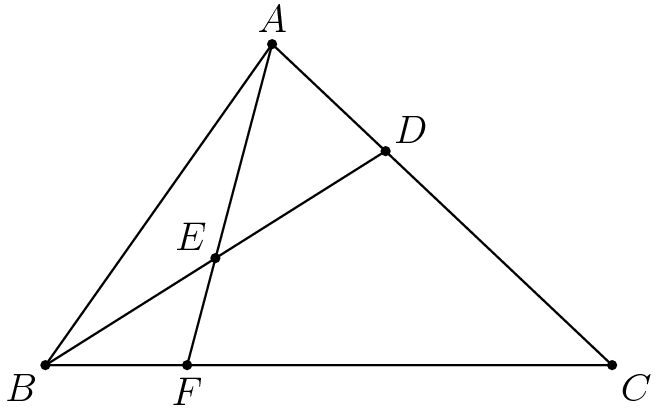
\includegraphics[width=4in]{images/mass_point_2019_AMC8_P24.png}
\end{center}

At first, the problem seemed innocuous: simple at best, a little bashy at worst. However, as I began frantically scribbling notes, the problem manifested itself as almost impossible. Coming out of the room, my annoyance was immeasurable; I quickly headed over to a consortium of the so-called “mathy” people of my school, three of whom got the answer: one by guessing, and the other two by drawing a very accurate diagram. But, still to all of us, the true method had yet to reveal itself.



During my next math class, our math teacher taught us a clever, and yet rarely taught, way to solve certain geometry problems that I want to share with you now; this method is called mass points, best taught through the example of that AMC 8 problem (admittedly, you could also solve it using triangle ratios, but mass points will annihilate the problem in under a minute). 
Below, in the problem statement, we have two crucial elements signifying that the method mass points might be viable: information about ratios and line intersections. Before we begin solving this problem, it’s important to note that the crux of mass points comes from physics: specifically, if you have two masses on a balance beam, they have to satisfy a special relationship for the beam to be balanced: taking either mass and multiplying it by the distance from that mass to the fulcrum (the “balance point” of the beam) gives you the same quantity. 

We can employ this property by using lines in the diagram as beams. For example, take $AC$: we know that $AD$ and $DC$ are in a 1 to 2 ratio, so we can assign $A$ and $C$ masses that make $AC$ a ``balanced beam'' (one of the great things about math as opposed to physics: you can just assign things). Theoretically, we could give them any mass, but, for simplicity’s sake, let’s just say that the mass of $A$ is 2 and the mass of $C$ is 1 (we can verify that this satisfies the “balancing act” we’re trying to fulfill: $A$ times $AD$ equals $C$ times $CD$). Great. Now what?

Another great property we can exploit in math (do not try this in your physics class) is to set the mass of $D$ to the mass of $A$ plus the mass of $C$, thereby setting it to 3. But, of course, this begs the question: why? Well, we want the entire diagram to be balanced and so we wish the line segment containing $D$ to be balanced, but this line segment will have $AC$ on one side and thus it has to balance all of $AC$, which is why we set D to the “total mass” of the line segment. And now the optimal strategy is to spam mass points until we’ve gotten the mass of every point we can, and hopefully we can find some ratio information that’s useful to us. 
In this problem, that approach looks something like this: we have that $D$ has mass 3 and the $E$ is the midpoint of $BD$; therefore, $B$ must have mass 3, and $E$ must have mass 6. Since we know that $A$ has mass 2, we can deduce that $F$ must have mass $6 - 2 = 4$ (you could confirm this by looking at $BC$ or $AF$). 

\begin{center}
    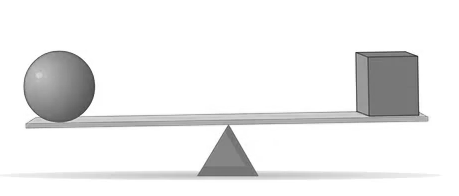
\includegraphics[width=4in]{images/mass-point.png}
\end{center}

Just from those simple calculations, we’ve deduced that $BF : FC = 1 : 3$, and $EF : EA = 1 : 2$. Thus $BF : BC = 1 : 4$ while $EF : AF  = 1 : 3$. This tells us that EBF's base is 4 times smaller than ABC’s and that its height is 3 times smaller (this is because their heights are in the same ratio as EF and AF). Therefore, the area of EBF must be $4 \cdot 3 = 12$ times smaller than ABC, so our answer is 30. 


While this problem may be simpler than most you will probably encounter in the future, I hope that it served as a good introduction to mass points–particularly, their simplification of laborious triangle-hunting (I think that’s a term). Before you go, I just want to remind you of when to use mass points. If you have ratio information and intersections, or you’re simply hunting for similar triangles on an easier problem, by all means use it; however, it’s unlikely that simple mass points will be enough for the likes of harder AMC 12 problems or beyond, so always try multiple methods, perhaps in conjunction. 
Mathematics is a field constructed out of basic elements that is rich in information and ripe for discovery, if only we are willing to tilt our heads in the right way--and that’s it for the math (and puns) from me!
\end{document}
